\documentclass[a3paper, 12pt]{article}

\usepackage[hscale=.9, vscale=.9]{geometry}
\usepackage{enumitem}
\usepackage{fix-cm}
\usepackage[none]{hyphenat}
\usepackage{graphicx}
\newcommand*\nfont{\fontsize{16}{19}\selectfont}

\parindent 0pt

%\hyphenation{distri-buted believe original other-wise}

\pagestyle{empty}

\begin{document}

% \vspace*{-5ex}
\begin{center}
  {\Huge Second International Workshop on}

  \medskip

  {\fontsize{36}{50}\selectfont Methods and Tools for Distributed
    Hybrid Systems}

  \bigskip

  {\Huge LIX, {\'E}cole polytechnique, Palaiseau, 4 July 2018}

  \medskip

  \bigskip

  \includegraphics[width=.8\linewidth]{lakeX2}

  \medskip
\end{center}

\begin{minipage}[t]{.47\linewidth}
  \nfont%
  The purpose of DHS is to connect researchers working in
  \emph{real-time} systems, \emph{hybrid} systems, \emph{control}
  theory, \emph{distributed} computing, and \emph{concurrency}, in
  order to advance the subject of \textbf{distributed hybrid systems}.

  \medskip

  Distributed hybrid systems, or distributed \emph{cyber- physical}
  systems, are abundant. Many of them are safety-critical, but
  ensuring their correct functioning is very difficult. We believe
  that new techniques are needed for the analysis and validation of
  DHS. More precisely, we believe that convergence and interaction of
  methods and tools from different areas of \emph{computer science},
  \emph{engineering}, and \emph{mathematics} is needed in order to
  advance the subject.

  \medskip

  The first DHS workshop was held in Aalborg, Denmark, in August 2017,
  featuring invited talks by Alessandro Abate, Martin Fr{\"a}nzle, Kim
  G.~Larsen, Martin Raussen, and Rafael Wisniewski. This second
  edition aims to continue the conversation.

  \bigskip

  {\Large \bf Call for Short Contributions}

  \smallskip

  We are calling for presentations of original, unfinished, already
  published, or otherwise interesting work which can highlight how the
  research topics of DHS may interact in order to advance the subject
  of distributed hybrid systems. Note that DHS 2018 will have no
  formal proceedings.

  \bigskip

  {\Large \bf Deadlines}

  \smallskip

  Submission of contributions: 10 June 2018

  Registration: 20 June 2018

  \bigskip

  {\Large \bf Organization}

  \smallskip

  Uli Fahrenberg, {\'E}cole polytechnique

  Alessandro Abate, Oxford University

  \vspace{13ex}

  {\Huge http:$/\!/$dhs.gforge.inria.fr/}

  \vspace*{-2ex}

\end{minipage}
\hfill
\begin{minipage}[t]{.45\linewidth}
  \nfont%
  \hfill {\Large \bf Invited Speakers}

  \smallskip

  \begin{minipage}{.2\linewidth}
    \includegraphics[width=\linewidth]{luc2}
  \end{minipage}
  \hfill
  \begin{minipage}{.75\linewidth}
    \textbf{Luc Jaulin}

    ENSTA Bretagne, Brest

    France
  \end{minipage}

  \vspace{-2ex}
  \begin{minipage}{.75\linewidth}
    \flushright%
    \textbf{Dmitry Kozlov}

    Universit{\"a}t Bremen

    Germany
  \end{minipage}
  \hfill
  \begin{minipage}{.2\linewidth}
    % \includegraphics[width=\linewidth, trim=60 0 0 0, clip]{kozlov2}
    \includegraphics[width=\linewidth]{kozlov2}
  \end{minipage}

  \vspace{-2ex}
  \begin{minipage}{.2\linewidth}
    \includegraphics[width=\linewidth]{thao}
  \end{minipage}
  \hfill
  \begin{minipage}{.75\linewidth}
    \textbf{Thao Dang}

    Verimag, Grenoble

    France
  \end{minipage}

  \vspace{-2ex}
  \begin{minipage}{.75\linewidth}
    \flushright%
    \textbf{Lisbeth Fajstrup}

    Aalborg Universitet

    Denmark
  \end{minipage}
  \hfill
  \begin{minipage}{.2\linewidth}
    \includegraphics[width=\linewidth]{fajstrup2}
  \end{minipage}

  \vspace{-2ex}
  \begin{minipage}{.2\linewidth}
    \includegraphics[width=\linewidth]{ledinot}
  \end{minipage}
  \hfill
  \begin{minipage}{.75\linewidth}
    \textbf{Emmanuel Ledinot}

    Dassault Aviation

    France
  \end{minipage}

  \vspace{-2ex}
  \begin{minipage}{.75\linewidth}
    \flushright%
    \textbf{Eric Goubault}

    {\'E}cole polytechnique

    France
  \end{minipage}
  \hfill
  \begin{minipage}{.2\linewidth}
    \includegraphics[width=\linewidth]{eric3}
  \end{minipage}

  \vspace{-2ex}
  \begin{minipage}{.2\linewidth}
    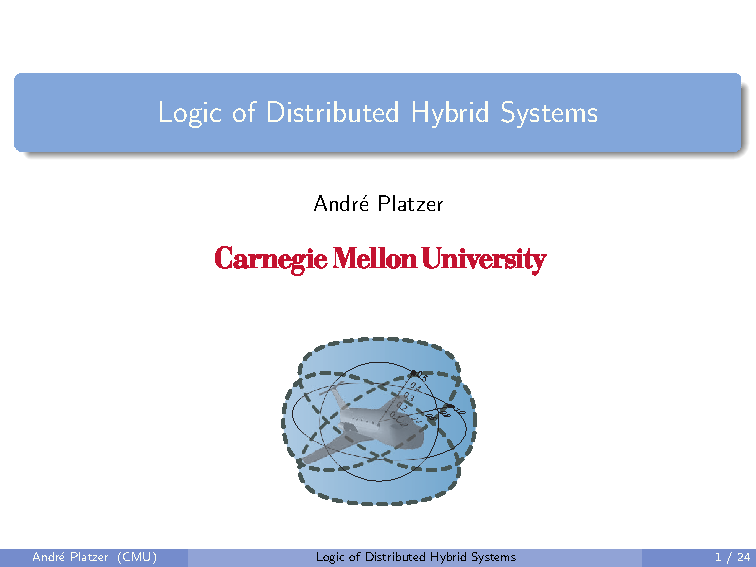
\includegraphics[width=\linewidth]{platzer}
  \end{minipage}
  \hfill
  \begin{minipage}{.75\linewidth}
    \textbf{Andr{\'e} Platzer}

    Carnegie Mellon University

    United States
  \end{minipage}

  \bigskip\bigskip

  \hspace*{-.15\linewidth}
  \begin{minipage}{1.15\linewidth}
    \hfill {\Large \bf Sponsors}

    \medskip

    \textbf{CISS} \hfill Center for Embedded Software Systems

    \hfill Aalborg, Denmark

    \smallskip

    \textbf{Chaire ISC} \hfill {\'E}cole polytechnique -- Thales -- FX

    \hfill DGA -- Dassault Aviation -- DCNS Research

    \hfill ENSTA ParisTech -- T{\'e}l{\'e}com ParisTech

    \hfill Paris, France

  \end{minipage}

\end{minipage}

\end{document}
